\documentclass{article}
% generated by Madoko, version 1.0.0-rc6
%mdk-data-line={1}


\usepackage[heading-base={2},section-num={False},bib-label={True}]{madoko2}


\begin{document}



%mdk-data-line={4}
\mdxtitleblockstart{}
%mdk-data-line={4}
\mdxtitle{\mdline{4}RBE 3002 Lab 4}%mdk
\mdxauthorstart{}
%mdk-data-line={9}
\mdxauthorname{\mdline{9}Keshuai Xu, William Sullivan, Richard Eberheim}%mdk
\mdxauthorend\mdtitleauthorrunning{}{}\mdxtitleblockend%mdk

%mdk-data-line={6}
\section{\mdline{6}1.\hspace*{0.5em}\mdline{6}Rviz screenshot}\label{sec-rviz-screenshot}%mdk%mdk

%mdk-data-line={7}
\noindent\mdline{7}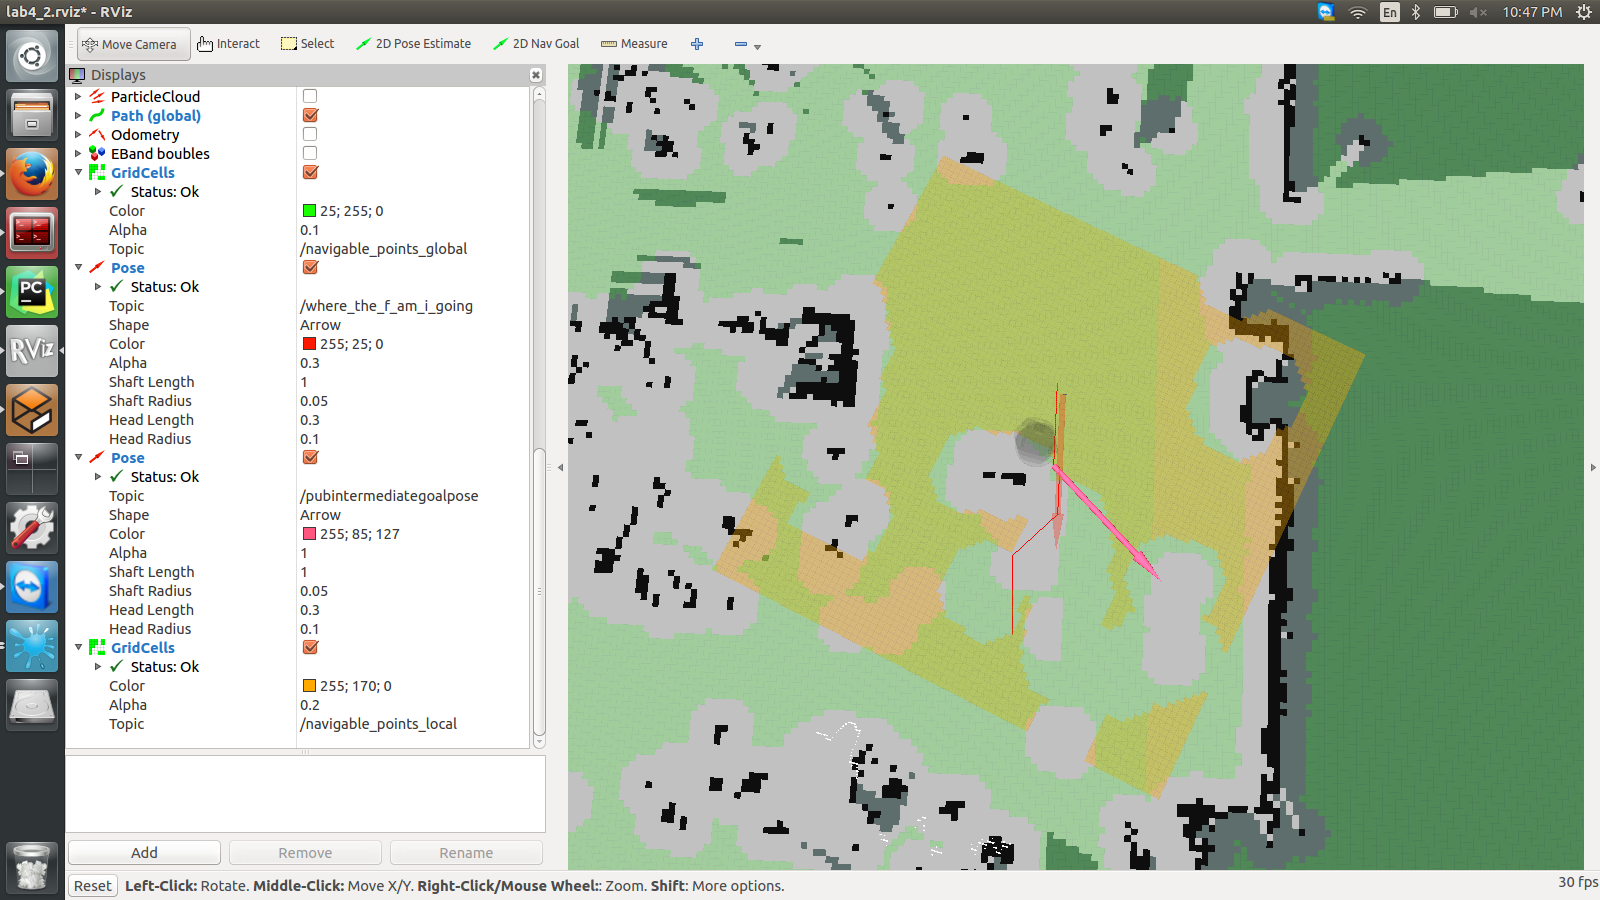
\includegraphics[keepaspectratio=true,width=\dimmin{}{\dimwidth{0.90}}]{images/Screenshot-from-2016-04-17-22-47-49}{}\mdline{7}%mdk

%mdk-data-line={11}
\noindent\mdline{11}The key for the map shown above is as follows:%mdk

%mdk-data-line={13}
\begin{itemize}[noitemsep,topsep=\mdcompacttopsep]%mdk

%mdk-data-line={13}
\item\mdline{13}The green cells are global navigable points.%mdk

%mdk-data-line={14}
\item\mdline{14}The orange cells are local navigable points.%mdk

%mdk-data-line={15}
\item\mdline{15}The red line is the global path planning.%mdk

%mdk-data-line={16}
\item\mdline{16}The blue line (not shown because no path was found) is the local path planning.%mdk
%mdk
\end{itemize}%mdk

%mdk-data-line={18}
\section{\mdline{18}2.\hspace*{0.5em}\mdline{18}Occupancy grid size}\label{sec-occupancy-grid-size}%mdk%mdk

%mdk-data-line={19}
\noindent\mdline{19}The occupancy grid size was not modified because our a-star algorithm is efficient enough to handle the original number of cells.%mdk

%mdk-data-line={21}
\mdline{21}The global and local costmap resolution is 0.05 m.%mdk

%mdk-data-line={23}
\section{\mdline{23}3.\hspace*{0.5em}\mdline{23}Updated heuristic}\label{sec-updated-heuristic}%mdk%mdk

%mdk-data-line={24}
\noindent\mdline{24}The new h-cost is the scaled-down weighed average of the Manhattan distance and the cost from the cost map.%mdk
\begin{mdpre}%mdk
\noindent{\mdcolor{darkgreen}\#~fr~and~to~are~tuples~(x,y)}\\
{\mdcolor{navy}def}~gethcost(fr,~to,~get\_cost\_map\_cost{\mdcolor{navy}=}{\mdcolor{navy}None}){\mdcolor{navy}:}\\
~~~~{\mdcolor{navy}if}~get\_cost\_map\_cost~{\mdcolor{navy}is}~{\mdcolor{navy}not}~{\mdcolor{navy}None}{\mdcolor{navy}:}\\
~~~~~~~~{\mdcolor{darkgreen}\#~magic~coefficients.~hopefully~the~added~cost~(0~to~10)~does~not~exceed~the~actual~distance}\\
~~~~~~~~{\mdcolor{navy}return}~gethcost(fr,~to)~*~{\mdcolor{purple}0.5}~+~get\_cost\_map\_cost(to)~*~{\mdcolor{purple}0.1}\\
~~~~{\mdcolor{navy}else}{\mdcolor{navy}:}\\
~~~~~~~~{\mdcolor{darkgreen}\#~manhattan~distance}\\
~~~~~~~~{\mdcolor{navy}return}~abs(to[{\mdcolor{purple}0}]~-~fr[{\mdcolor{purple}0}])~+~abs(to[{\mdcolor{purple}1}]~-~fr[{\mdcolor{purple}1}])%mdk
\end{mdpre}
%mdk-data-line={36}
\section{\mdline{36}4.\hspace*{0.5em}\mdline{36}Reading the cost map}\label{sec-reading-the-cost-map}%mdk%mdk

%mdk-data-line={37}
\noindent\mdline{37}In class \mdline{37}\mdcode{CostmapThing}\mdline{37}, two callback functions were written to handle the cost map update. We subscribed to the \mdline{37}\mdcode{\textasciitilde{}costmap}\mdline{37} and \mdline{37}\mdcode{\textasciitilde{}costmap\_updates}\mdline{37} of both local and global cost map to maintain updated copies of the cost maps. The cost maps were then binarized with a set threshold to determine the navigable area when a-star path planning is called.%mdk

%mdk-data-line={39}
\section{\mdline{39}5.\hspace*{0.5em}\mdline{39}A-star path planning}\label{sec-a-star-path-planning}%mdk%mdk

%mdk-data-line={40}
\noindent\mdline{40}The path planning is done in array index unit in the corresponding map\mdline{40}'\mdline{40}s frame. The array indicies were converted to the coordinate in the the map\mdline{40}'\mdline{40}s frame when generating the waypoints.T he waypoints were transformed into \mdline{40}\mdcode{/map}\mdline{40} frame before feeding into the move base function. \mdline{40} \mdline{40}%mdk

%mdk-data-line={42}
\section{\mdline{42}6.\hspace*{0.5em}\mdline{42}Path planning logic}\label{sec-path-planning-logic}%mdk%mdk

%mdk-data-line={43}
\noindent\mdline{43}The program does an initial planning in global map, then plan in local repetitively to go to the global waypoints until reaches the goal. If no path found in local, the program replan the path in global.%mdk

%mdk-data-line={45}
\mdline{45}The local path planning handles dynamic obstacles.%mdk

%mdk-data-line={47}
\begin{itemize}[noitemsep,topsep=\mdcompacttopsep]%mdk

%mdk-data-line={47}
\item\mdline{47}In a while loop, search in the global map with a-star. If there is a path, extract the first waypoint.

%mdk-data-line={48}
\begin{itemize}[noitemsep,topsep=\mdcompacttopsep]%mdk

%mdk-data-line={48}
\item\mdline{48}If it is the global goal, mark done and exit the loop after finishing rest of the code.%mdk

%mdk-data-line={49}
\item\mdline{49}try to find a path in local map from the current pose to first waypoint in global map (local goal), with maximum distance of 1m. 

%mdk-data-line={50}
\begin{itemize}[noitemsep,topsep=\mdcompacttopsep]%mdk

%mdk-data-line={50}
\item\mdline{50}If path is found, execute the path. 

%mdk-data-line={51}
\begin{itemize}[noitemsep,topsep=\mdcompacttopsep]%mdk

%mdk-data-line={51}
\item\mdline{51}If next waypoint is local goal, navigate to it and replan in global.%mdk
%mdk
\end{itemize}%mdk%mdk

%mdk-data-line={52}
\item\mdline{52}If no path is found, plan in global again. If still no path found, give up.%mdk
%mdk
\end{itemize}%mdk%mdk
%mdk
\end{itemize}%mdk%mdk

%mdk-data-line={53}
\item\mdline{53}If no path found initially in global map, give up.%mdk
%mdk
\end{itemize}%mdk

%mdk-data-line={55}
\section{\mdline{55}7.\hspace*{0.5em}\mdline{55}Move the base}\label{sec-move-the-base}%mdk%mdk

%mdk-data-line={56}
\noindent\mdline{56}We created a version of the \mdline{56}\mdcode{navToPose()}\mdline{56} function that does not turn to the goal orientation when reaches the goal to use in the intermediate steps in local path following to save time. The robot only turn to goal orientation when it reaches the global goal.%mdk%mdk


\end{document}
